\documentclass[../../main.tex]{subfiles}
% \graphicspath{{\subfix{../images/}}}

\begin{document}
Como mencionamos anteriormente, las redes neuronales convolucionales (RNCs) son un tipo
especializado de redes neuronales pensadas para el procesamiento de datos que tienen una
estructura de grilla \cite{deep-learning}. Ejemplos de estos datos son las series de
tiempo, que pueden pensarse como una grilla unidimensional, y las imágenes, que pueden
verse como una grilla bidimiensional de píxeles.

Si bien las RNCs se han usado principalmente para el procesamiento de imágenes, en este
trabajo nos enfocaremos en su uso para analizar series de tiempo, en particular
unidimensionales. Veremos cómo su funcionamiento permite capturar patrones temporales en
los datos.

Una \textbf{serie de tiempo univariada o unidimensional} se puede representar como un
vector ordenado \(U\) de valores reales que reflejan la evolución a lo largo del tiempo
de un determinado fenómeno:
\[
    U = (x_1, x_2, ..., x_N)
\]
donde \(N\) es la cantidad total de observaciones, y \(x_i\) corresponde el valor observado
en el período \(i\), para \(i = 1,...,N\).

Las series de tiempo están presentes en una gran variedad de situaciones de la realidad.
Algunos ejemplos incluyen la evolución del precio de un activo financiero, la variación de
indicadores de salud como el ritmo cardíaco, los registros diarios de temperatura y
precipitaciones, el seguimiento de indicadores económicos o sociales como la tasa de
empleo o niveles de pobreza, entre muchos otros. En el contexto de este trabajo, estas
series se utilizarán como entradas de las redes neuronales.

El término \textit{convolucionales} proviene del hecho que lo que caracteriza a estas
redes es la utilización de una operación matemática llamada
\textbf{convolución}\footnote{En realidad, la operación que está presente en estas redes
es una relacionada con la convolución, llamada \textbf{correlación cruzada}, pero el
término que se utiliza sigue siendo convolucionales. El símbolo que se suele utilizar es
\(\ast\).} \cite{deep-learning}. Las capas de la red que aplican esta operación son
llamadas \textit{capas convolucionales}.

La convolución toma dos argumentos: por un lado, la \textit{entrada} y por otro lado, un
\textit{filtro} o \textit{kernel}. En el contexto del ML, ambos son usualmente arreglos
multidimensionales de números reales, también comúnmente llamados tensores
\cite{deep-learning}. Intuitivamente, la operación consiste en ``deslizar'' el filtro
sobre la entrada, y en cada momento calcular el producto escalar. Para verlo más
claramente en el caso unidimensional, tomemos un ejemplo.

Dado como entrada a la convolución un vector\footnote{Por conveniencia, el primer elemento
de los vectores será indexado en 1, y no en 0.} \(\bm{x} = (x_1, x_2, ..., x_m)\ (m \in
\mathbb{N})\), si tomamos un filtro de tamaño 3, dado por \(\bm{w}=(w_1, w_2, w_3)\),
entonces el resultado de la convolución es un vector \(\bm{z}\) en donde cada componente
\(z_i\) es una suma pesada de las entradas ``cercanas'' a \(x_i\):
\[z_i = w_1 x_{i-1} + w_2 x_{i} + w_3 x_{i+1}\]


En la Figura \ref{fig:conv1d-example}, se puede ver cómo se computan \(z_2\) y \(z_3\) en
un ejemplo en donde la entrada es de tamaño 6 y el filtro de tamaño 3. Un detalle a notar
aquí es que al calcular \(z_2\) y \(z_3\), el filtro ``entra'' por completo en una región
de la entrada, pero si quisiéramos calcular \(z_1\), pareciera que \(w_1\) no tiene un
valor de entrada con el cual multiplicarse. Existen alternativas para solucionar este
problema que detallaremos más adelante.

\begin{figure}
    \centering
    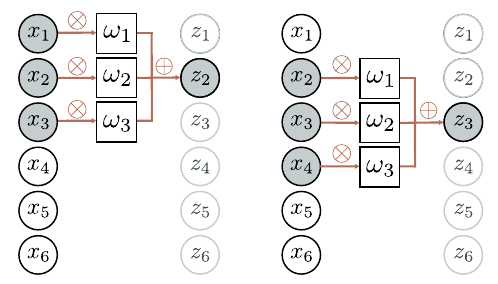
\includegraphics[width=0.55\textwidth]{figs/conv1d-example1.png}
    \caption{Fuente: \cite{prince2024understanding}. Ejemplo de convolución unidimensional
    aplicada sobre una entrada de tamaño 6 con un filtro \(\bm{w} = (w_1, w_2, w_3)\) de
    tamaño 3. El símbolo \(\otimes\) indica la multiplicación, y el \(\oplus\) la suma.}
    \label{fig:conv1d-example}
\end{figure}

Si generalizamos y tomamos un vector \(\bm{x}\) de tamaño \(n\) correspondiente
a la entrada y un vector \(\bm{w}\) de tamaño \(l\) correspondiente al kernel,
entonces el resultado de la convolución es un vector \(\bm{z}\) donde:
\begin{equation}
    z_i = \sum_{j=1}^l w_j x_{j+i-(l+1)/2}
    \label{eq:convolution}
\end{equation}
En otras palabras, para generar cada componente \(i\) de la salida, se toma el producto
escalar entre el kernel \(\bm{w}\) y una parte de \(\bm{x}\) de largo \(l\) centrada en
\(x_i\) \cite{ai-a-modern-approach}.

La salida de la convolución suele llamarse \textbf{mapa de características}
(\textit{feature map}) \cite{deep-learning}, y resalta las áreas de la entrada que son
``similares'' a la característica que el filtro está tratando de capturar
\cite{hands-on-ML-sklearn-tf}. Para ver esto, tomemos otro ejemplo.

Supongamos que tenemos el filtro \(\bm{w} = (1, 0, -1)\) (de tamaño \(l=3\)). Entonces,
usando la Ecuación \ref{eq:convolution}, veamos qué calcula este filtro en cada
posición \(i\) de la salida:
\begin{align*}
    z_i &=\ \sum_{j=1}^3 w_j x_{j+i-(3+1)/2} \\
        &=\ \sum_{j=1}^3 w_j x_{j+i-2} \\
        &=\ w_1 x_{1+i-2} + w_2 x_{2+i-2} + w_3 x_{3+i-2} \\
        &=\ 1 \cdot x_{i-1} + 0 \cdot x_i + (-1) \cdot x_{i+1} \\
        &=\ x_{i-1} - x_{i+1}
\end{align*}
O sea, dada una posición \(i\) en la entrada \(\bm{x}\), el filtro calcula la diferencia
entre el ``vecino'' izquierdo (\(x_{i-1}\)) y el derecho (\(x_{i+1}\)). De esta forma, si
para un \(i\) el valor resultante de aplicar el filtro es positivo, quiere decir que hubo
una transición de un valor mayor a uno menor (una ``bajada''), y si es negativo, viceversa
(una ``subida''). Si el valor es cercano a 0, significa que la entrada no cambia
signficativamente de valor entre los dos vecinos. En este caso, se podría decir que el
filtro ``detecta'' regiones de la entrada en donde hay aumentos o descensos. Este ejemplo
se puede ver más claramente en la Figura \ref{fig:conv-example}.

\begin{figure}
    \centering
    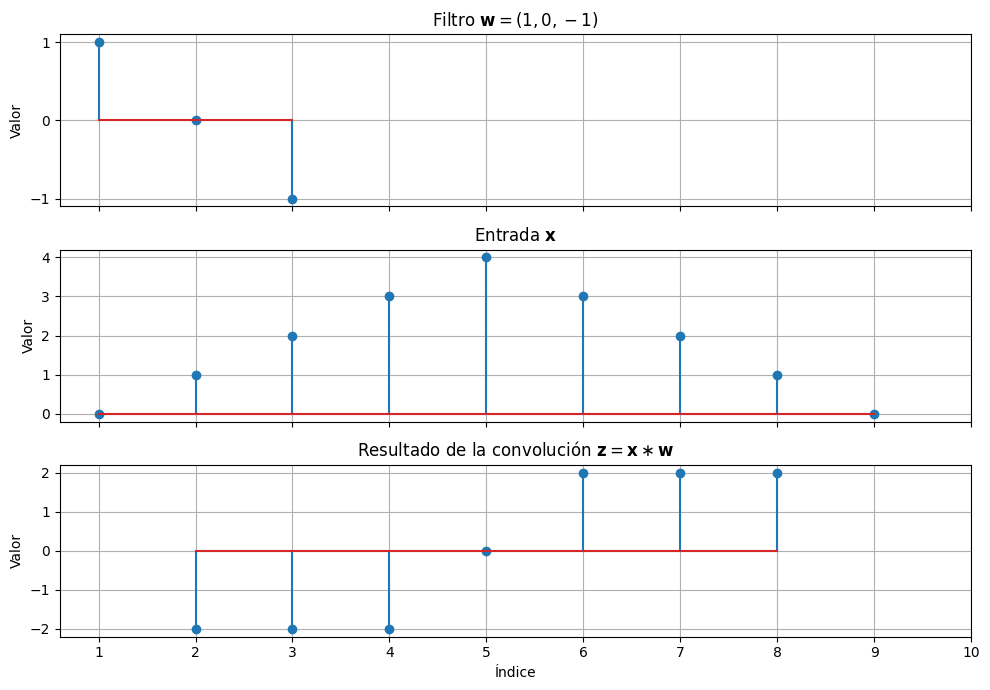
\includegraphics[width=0.55\textwidth]{figs/ejemplo_convolucion.png}
    \caption{Ejemplo de convolución unidimensional en donde se aplica el filtro \(\bm{w} =
    (-1,0,1)\) sobre una entrada de tamaño 9. El resultado de la convolución se calcula
    únicamente en aquellas posiciones donde el filtro puede superponerse completamente con
    la entrada. Se puede ver que en las regiones donde los valores vecinos presentan un
    aumento o descenso, el resultado de la convolución es distinto de 0. En cambio, en
    la posición 5, donde los vecinos tienen el mismo valor, el resultado es 0.}
    \label{fig:conv-example}
\end{figure}

A partir de esto, podemos ver que cada filtro se encarga de identificar una característica
específica en la entrada, y que dicha característica depende de los valores del filtro. En
las RNCs, estos valores — los pesos involucrados en cada filtro — son justamente los
parámetros a optimizar durante el proceso de entrenamiento. El objetivo es que el modelo
aprenda exactamente qué filtros le son más útiles para capturar los rasgos relevantes
presentes en los datos.

Para entender cómo se aplican estos filtros en las RNCs, es importante describir el
funcionamiento de las capas convolucionales, que son las responsables de realizar la
operación de convolución. A diferencia de las redes totalmente conectadas, donde cada
neurona de una capa está conectada con todas las de la capa anterior, lo que ocurre en las
capas convolucionales es que cada neurona se conecta únicamente con un subconjunto de
neuronas (consecutivas) de la capa anterior. Este subconjunto recibe comúnmente el nombre
de \textbf{campo receptivo} y es sobre el que cada neurona aplicará el filtro
correspondiente. Por ejemplo, en la Figura \ref{fig:conv1d-example}, si vemos a la columna
de la izquierda como las entradas, y la de la derecha como una capa convolucional, el
campo receptivo de la neurona \(z_2\) está formado por \(x_1\), \(x_2\) y \(x_3\), y el de
la neurona \(z_3\) por \(x_2\), \(x_3\) y \(x_4\).

Además, es importante notar que cada neurona de una capa convolucional aplica el mismo
filtro, por lo que todas las neuronas de una misma capa comparten los mismos pesos. Esto
se puede observar claramente en la Figura \ref{fig:conv1d-example}, donde tanto la neurona
\(z_2\) como la \(z_3\) aplican el mismo filtro (\(w_1, w_2, w_3\)) sobre sus respectivos
campos receptivos. Como consecuencia, la cantidad de parámetros a aprender en una red
convolucional es menor que en una red totalmente conectada. Esta diferencia puede verse en
la Figura \ref{fig:fully-connected-vs-conv}.

\begin{figure}
    \centering
    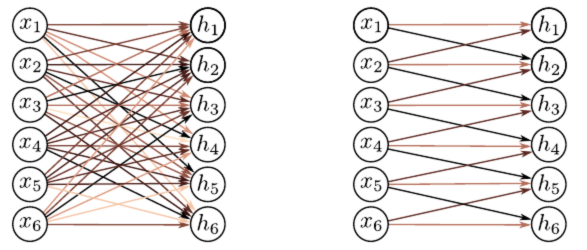
\includegraphics[width=0.55\textwidth]{figs/fully-connected-vs-conv.png}
    \caption{Fuente: \cite{prince2024understanding}. Capas de una red totalmente conectada
    (izquierda) y capas convolucionales (derecha). Denotamos con \(x\) a la capa de la
    izquierda, y con \(h\) a la de la derecha, en ambos casos. En la arquitectura
    totalmente conectada, cada neurona de la capa \(x\) está conectada con todas las
    neuronas de la capa \(h\), habiendo un total de \(6 \cdot 6 = 36\) pesos entre ellas.
    En cambio, en la convolucional, asumiendo que se aplica un filtro de tamaño \(l=3\),
    cada neurona de la capa \(h\) computa una suma pesada de \(l=3\) neuronas consecutivas
    de la capa \(x\), usando los mismos pesos. Esto reduce la cantidad de parámetros entre
    ambas capas de 36 a 3.}
    \label{fig:fully-connected-vs-conv}
\end{figure}

Con esta idea de campo receptivo, podemos pensar en una red con dos capas convolucionales
consecutivas, donde cada neurona aplica un filtro de tamaño 3. Lo que va a ocurrir
entonces es que las neuronas de la primera capa oculta toman una suma pesada sobre
conjuntos de 3 neuronas consecutivas de la capa de entrada. Luego, las unidades de la
segunda capa oculta hacen lo mismo sobre conjuntos de 3 neuronas consecutivas de la
primera capa oculta, que a su vez ya representan combinaciones locales de la entrada. Esto
implica que la primera capa oculta se concentra en características de bajo nivel, más
específicas, mientras que las capas posteriores aprenden representaciones progresivamente
más abstractas como resultado de integrar los patrones detectados en las capas anteriores
\cite{hands-on-ML-sklearn-tf}.

Hasta ahora vimos una capa convolucional que aplica solamente un filtro, lo que nos va a
dar como resultado solamente un mapa de características. Sin embargo, una misma capa puede
aplicar varios filtros (todos del mismo tamaño), cada uno de los cuales va a generar su
propio mapa de características. Para esto, lo que se hace es darle a la capa una
``profundidad'' de tantos filtros como querramos aplicar sobre la entrada, obteniendo de
esta forma un mapa para cada nivel profundidad, cada uno capturando una característica
puntual de la entrada. Así, se suele decir que una capa tiene varios \textit{canales}.

Algo que cabe notar en este punto es que cuando una neurona aplica el filtro
correspondiente sobre las de la capa anterior, si esta última tiene varios canales,
entonces el filtro es aplicado en todos ellos. Es decir, si la capa anterior tiene \(C\)
canales y el filtro tiene tamaño \(l\), entonces al aplicarlo, ahora va a haber una
cantidad de pesos \(l \cdot C\). Esto se puede ver en la Figura
\ref{fig:conv-layer-multi-channel}.

\begin{figure}
    \centering
    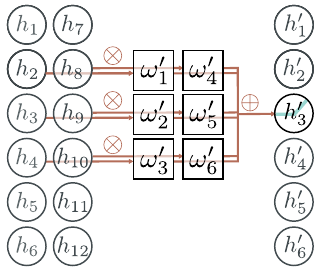
\includegraphics[width=0.35\textwidth]{figs/conv-layer-multi-channel.png}
    \caption{Fuente: \cite{prince2024understanding}. La capa de neuronas \(h_i\) tiene
    dos canales: aquel formado por las neuronas \(h_1\) a \(h_6\) y aquel formado
    por las neuronas \(h_7\) a \(h_{12}\). La capa de neuronas \(h'_i\) aplica un
    filtro de tamaño \(l=3\) sobre cada uno de los canales de la capa anterior. Por
    lo tanto ahora termina habiendo \(2 \cdot 3 = 6\) pesos entre cada neurona de la
    capa \(h'_i\) y la capa \(h_i\).}
    \label{fig:conv-layer-multi-channel}
\end{figure}

Además de la cantidad de filtros en una capa, y su tamaño \(l\), existen otros
hiperparámetros de las capas convolucionales: \vspace{-0.25cm}
\begin{itemize}[noitemsep]
    \item El \textbf{paso} (\textit{stride}), que representa la distancia entre dos campos receptivos
    consecutivos. Un stride igual a 1 quiere decir que el filtro se aplica en cada
    posición de la entrada.
    \item El \textbf{relleno} (\textit{padding}), que controla cuántos valores
    ``fantasma'' se agregan artificialmente a los extremos de la entrada de forma tal que
    el tamaño de la salida de la convolución no sea tanto menor al de la entrada. En la
    práctica, se suele usar el 0 para este relleno (\textit{zero-padding}). Con esto, se
    puede computar el valor de \(z_1\) que presentamos en la Figura
    \ref{fig:conv1d-example}.
    \item La \textbf{dilatación} (\textit{dilation}), que determina cuántos 0s se
    intercalan en los pesos del filtro. Con este parámetro, se puede convertir un filtro
    de \(l=5\) a uno ``dilatado'' de tamaño 3 fijando el segundo y cuarto elementos en 0.
    Esto permite seguir ``integrando'' la información de una región de la entrada de
    tamaño 5 pero requiriendo solamente 3 pesos para hacerlo
    \cite{prince2024understanding}.
\end{itemize}

Otros de los componentes particulares de las RNCs son las capas de
\textbf{\textit{pooling}}, cuyo objetivo principal es reducir el tamaño del mapa producido
por la convolución \cite{hands-on-ML-sklearn-tf}. Es decir, se aplican luego de la
convolución y lo que hacen es reemplazar valores contiguos presentes en una determinada
sección del mapa por una medida resumen de ellos, entre las cuales algunas comúnmente
utilizadas son el máximo (\textit{max pooling}) y el promedio (\textit{average pooling}).

De esta forma, una capa convolucional típica de una RNC se compone de tres etapas: en
primer lugar, se producen las convoluciones, que se encargan de producir activaciones
lineales; luego, cada una de estas activaciones pasa por una función de activación no
lineal; y finalmente se aplica pooling para reducir el tamaño de la salida
\cite{deep-learning}. Y así, una RNC profunda se compone de varias de estas capas.

\medskip
Una técnica particular que ha demostrado tener un efecto positivo al entrenar redes
convolucionales es una conocida como \textbf{normalización de lote} (\textit{batch
normalization}) \cite{batch-norm} \cite{deep-learning} \cite{hands-on-ML-sklearn-tf},
introducida en 2015. Esta consiste en reescalar los valores generados en las capas
intermedias de la red a partir de los ejemplos en el lote actual
\cite{ai-a-modern-approach}. La normalización suele agregarse antes de la aplicación de la
función de activación y es importante notar que agrega nuevos parámetros a optimizar
durante el entrenamiento de la red. Para ver los detalles concretos de esta técnica, se
puede consultar el Capítulo 11 de \cite{hands-on-ML-sklearn-tf}.

\bigskip
En este trabajo, empleamos este tipo de redes para resolver la tarea de
\textbf{clasificación de series de tiempo}. Esto es: dada una serie de tiempo como entrada
de la red, se busca que la red sea capaz de predecir a qué categoría corresponde. Para
ello, lo que se suele hacer es aplanar (\textit{flatten}) la salida de la última capa
convolucional. Esta operación simplemente convierte el tensor resultante de dicha capa en
uno unidimensional, por lo que no agrega nuevos parámetros aprendibles durante el
entrenamiento. Por ejemplo, si la salida consiste de \(k\) mapas de características de
longitud \(n\) cada uno, entonces aplanarla dará como resultado un vector unidimensional
de tamaño \(k \times n\).

El paso anterior es necesario ya que las capas siguientes que se agregan para hacer la
clasificación son totalmente conectadas que, como vimos anteriormente, aceptan únicamente
entradas unidimensionales. Entonces, lo que ocurre es que el vector de tamaño \(k \times
n\) es procesado por estas últimas hasta finalmente llegar a la de salida.

En problemas de clasificación con más de dos categorías, la capa de salida suele tener
tantas neuronas como clases haya. Sin embargo, para tareas de clasificación binaria, como
la que tratamos aquí, se utiliza habitualmente una única neurona con una función de
activación sigmoide, cuya salida representa la probabilidad de que la secuencia de entrada
pertenezca a la clase positiva (usualmente asociada con la etiqueta 1).

\end{document}